\section{Sugar refining, 1890--1914: Genesove and Mullin (1998)}\label{sec:03-sugar}

The methods of \cref{sec:03-sumner,sec:03-identification} infer market power without observing marginal
cost. Their answers are only as good as the maintained assumptions on demand, cost and conduct. Whether
those assumptions deliver the right answer in a real industry is an empirical question.
\citet{GenesoveMullin1998} answer it for American cane sugar refining between 1890 and 1914, an industry in
which marginal cost can be measured almost directly. They compute conduct twice. The first computation uses
the cost information and serves as a benchmark. The second treats cost as unknown and applies the standard
estimator of the New Empirical Industrial Organization (NEIO). Together with the electricity study of
\cref{sec:03-electricity}, this comparison is the closest the literature comes to a controlled test of the
conduct-parameter method.\footnote{We work from two versions. The article \citep{GenesoveMullin1998} is
cited by its table numbers (``Table 2'') and its published page numbers. The working paper \citep{GenesoveMullin1995} contains a longer
history, the cost evidence and several tables that the article omits. We cite those as ``WP Table 9'' and
give its printed page numbers. Published Tables 2, 3 and 4 correspond to WP Tables 4, 6, and 7 and 8.
Published Table 10 reproduces two columns of WP Table 14 with a different direct measure. Published Table 9
has no counterpart in the working paper.}

\subsection{The question and why sugar}\label{sec:03-sugar-question}

Genesove and Mullin start from the supply relation \eqref{eq:03-supply-relation} with a constant marginal
cost $c$,
\begin{equation}\label{eq:03-gm-supply}
P + \theta\, Q\, P'(Q) = c ,
\end{equation}
and from its Lerner form \eqref{eq:03-lerner-theta}, $\theta = \varepsilon(P)\frac{P - c}{P} \equiv
L_\varepsilon$. With complete cost information and an estimated demand elasticity, the elasticity-adjusted
Lerner index delivers $\theta$ period by period. Without cost information, $\theta$ must be restricted,
because an unrestricted $\theta_t$ fits any data (\cref{prop:03-exact-fit}). The usual restriction is that
$\theta$ is constant, or at least uncorrelated with the instruments (WP p.~4).

Three features make sugar refining the right place for a test (WP pp.~3--4). First, the technology is
simple. Raw sugar is turned into refined sugar at a fixed and known coefficient, both prices are observed,
and the remaining costs are documented. A true price-cost margin can therefore be computed. Second, the
harvest cycle of raw sugar and year-to-year weather generate supply variation that is plausibly exogenous to
American demand. This variation helps identify demand and, through it, conduct. Third, the industry went
through dramatic structural changes: the formation of a trust, repeated entry with price wars, renewed
consolidation, and an antitrust prosecution. These episodes let us ask whether estimated conduct moves with
structure, and whether the method can tell a change in conduct from a change in cost.

The test answers two standing objections to the NEIO (WP pp.~2--3). The first is that functional forms for
demand impose strong restrictions on the relation between price and marginal cost. The second is the point
of \citet{Corts1999} developed in \cref{sec:03-corts}. The estimated conduct parameter measures the marginal
response of the markup to the identifying shocks, and so may misstate its level. Genesove and Mullin note
that no NEIO estimate had ever been checked against an independent measure of conduct. Their design makes
three comparisons. The NEIO estimate $\hat\theta$ is compared with the direct measure $L_\varepsilon$. The
NEIO estimates of the cost parameters are compared with their documented values. Finally, the estimates for
different structural regimes are compared with the direct measures for the same regimes. Throughout, the
maintained hypothesis is that $L_\varepsilon$ measures conduct without error (WP p.~5).

\subsection{The industry, 1887--1914}\label{sec:03-sugar-history}

The American cane sugar refining industry of this period combined high concentration with repeated entry.
\Cref{tab:03-gm-chronology} lists the main events (WP Tables 1 and 13). The account below follows WP
pp.~6--8 and 13--15. These pages rely on \citet{Eichner1969}, \citet{Zerbe1969} and Willett and Gray's
\emph{Weekly Statistical Sugar Trade Journal}, the source of most of the data.

\begin{table}[htbp]
\centering
\caption{Chronology and structural regimes of the U.S. sugar refining industry}\label{tab:03-gm-chronology}
\small
\begin{tabular}{@{}ll@{}}
\toprule
\multicolumn{2}{@{}l}{\textit{Panel A. Events (WP Table 1 and text)}}\\
\midrule
1887 (Dec.) & Sugar Trust formed: 18 firms with 80 percent of capacity\\
1889--1890 & Entry by Spreckels (Philadelphia plant completed in Dec. 1889), price war\\
1891 & Trust reorganized as the American Sugar Refining Company (ASRC)\\
1891--1892 & Acquisition of Spreckels and others, ASRC reaches 95 percent of capacity\\
1892--1896 & Small-scale entry by five single-plant firms, cartel operation\\
1898 & Entry by Arbuckle Brothers (August) and Doscher (November)\\
1900 (May) & End of the Arbuckle war\\
1903 & Cuban Reciprocity Treaty: Cuban raw sugar enters at 80 percent of full duty\\
1910 & Federal antitrust suit (consent decree in 1922)\\
1914 & World War I begins, the sample ends in June 1914\\
\midrule
\multicolumn{2}{@{}l}{\textit{Panel B. Regimes used in the estimation (WP Table 13)}}\\
\midrule
Jan. 1890 to Feb. 1892 & Spreckels entry, price war\\
Mar. 1892 to Sep. 1898 & Acquisition of Spreckels, small-scale entry, cartel operation\\
Sep. 1898 to Apr. 1900 & Entry by Arbuckle Brothers and Doscher, price war\\
May 1900 to 1910 & After the Arbuckle war\\
Nov. 1910 to 1913 & Government antitrust suit\\
\bottomrule
\end{tabular}

\smallskip
\begin{minipage}{0.92\textwidth}\footnotesize
Notes: Compiled from \citet{GenesoveMullin1995}, WP Tables 1 and 13 and pp.~6--8. The two price-war regimes
in Panel B are the ``post-entry price wars'' of \cref{sec:03-sugar-wars}.
\end{minipage}
\end{table}

\casehead{Trust and first entry}
After several failed attempts at collusion, the Sugar Trust was formed in December 1887. It consolidated 18
firms that controlled 80 percent of industry capacity, and it soon reduced their 20 plants to 10. The
average refined price rose about 16 percent, from \$6.013 per hundred pounds in 1887 to \$7.007 in 1888 (WP
p.~6, fn.~2). Entry followed. Claus Spreckels, a West Coast refiner, completed a plant in Philadelphia in
December 1889, in retaliation for the Trust's purchase of a California refinery. A price war ensued. The
Trust, reorganized in 1891 as the American Sugar Refining Company (ASRC), then bought the Spreckels plant
and the remaining outsiders. By April 1892 it held 95 percent of capacity. Genesove and Mullin describe this
episode as the template for the period: high concentration, punctuated by entry, price wars, and then
acquisition of or accommodation with the entrants (WP p.~7).

\casehead{Cartel and second entry}
Between 1892 and 1896 five firms entered, each with a single plant of about 1,340 barrels of refined sugar
per day on average. ASRC and its ``friendly'' companies had 49,500 barrels per day. ASRC acted as cartel
leader, and by 1896 an understanding with the independents had evolved. The next challenge came from the
Arbuckle Brothers, wholesale grocers and the dominant American coffee roasters. Their refinery began limited
production in August 1898, and the Doscher refinery started in November. Each plant had a capacity of 3,000
barrels per day. A severe price war followed, with pricing at or below cost, shutdowns by independent
refiners and partial exit of one entrant. Apart from one respite, the war lasted until May 1900. It ended
when Doscher merged with two major independents in a transaction organized by the president of ASRC (WP
pp.~7--8).

\casehead{Tariffs, antitrust and fringes}
The tariff on refined sugar protected domestic refiners from European competition. From 1903, the Cuban
Reciprocity Treaty admitted Cuban raw sugar at 80 percent of the full duty. In antitrust, the government
challenged ASRC's purchase of several Philadelphia refineries in 1892, and the Supreme Court upheld the
acquisition in 1895 (the \emph{E.\,C.~Knight} case). In 1910 the federal government sued for dissolution.
The case ended in a consent decree only in 1922, but after the government's victories against Standard Oil
and American Tobacco in 1911, ASRC began a partial ``voluntary'' dissolution (WP p.~8). Two competitive
fringes disciplined the cane refiners. Domestic beet sugar supplied less than 1 percent of consumption until
1894, 5 percent by 1901 and 15 percent in 1908--1914. European beet refiners were a threat of imports, and
ASRC's president testified in 1888 and 1894 that ASRC set prices so that no refined sugar would be imported
(WP p.~14). Genesove and Mullin do not model the fringes. Their conduct measures are therefore ``overall''
measures that include the discipline of potential imports and beet sugar (WP p.~15).

\casehead{Product, sunk costs and capacity}
The standard grade of refined sugar, ``standard granulated,'' was a homogeneous product. Refiners shipped it
to grocers in barrels, and grocers repackaged it without identifying the manufacturer, so prices tended to
uniformity (WP pp.~13--14). A refinery of 3,000 barrels per day cost between \$1.5 and \$2.5 million in 1900.
Plant and machinery had little value outside sugar, while the waterfront land had considerable salvage value.
Entry costs were thus largely, but not completely, sunk. Industry output stayed well below capacity
throughout, and ASRC kept excess capacity even in the depths of the Arbuckle war (WP p.~13). ASRC's share
of the market fell from 91 percent in 1892 to 43 percent in 1914 (WP Table 9).

\subsection{Technology and the direct measurement of marginal cost}\label{sec:03-sugar-cost}

Refined sugar was made mostly from cane. Cane was first processed into raw sugar, which could be shipped
and stored. The standard grade, ``96 degree centrifugals,'' was 96 percent sucrose, and its sugar content
was tested with a polariscope, which made the input homogeneous. Most raw sugar came from the tropics,
especially Cuba, with Louisiana the main domestic source. Refiners melted, purified and crystallized it
into refined sugar, which is pure sucrose. Witnesses for both ASRC and an independent testified that all
refiners used a common process (WP p.~9).

\begin{assumption}[Fixed-coefficient technology]\label{ass:03-gm-cost}
The marginal cost of producing one hundred pounds of refined sugar in period $t$ is
\begin{equation}\label{eq:03-gm-cost}
c_t = c_0 + k\,P^{\mathrm{raw}}_t .
\end{equation}
Here $P^{\mathrm{raw}}_t$ is the price of one hundred pounds of raw sugar, and $k$ is the quantity of raw sugar
needed per unit of refined sugar. The term $c_0$ collects all other variable costs (labor, fuel, boneblack,
packages, brokerage, net of the value of byproducts). Both $c_0$ (in constant dollars) and $k$ are constant
over time and do not depend on output.
\end{assumption}

The assumption that marginal cost does not depend on output is natural in an industry that always operated
well below capacity. Genesove and Mullin maintain \eqref{eq:03-gm-cost} throughout, and then measure $k$ and
$c_0$ from engineering and testimonial evidence.

\casehead{The input coefficient}
Raw sugar is 96 percent sucrose, so the physical minimum is $k = \frac{1}{0.96} = 1.042$. The working paper
truncates this value and prints 1.041 (WP p.~10). Some sugar is lost
in refining. A Treasury commission found in 1898 that one hundred pounds of raw sugar yielded 92.5 pounds of
refined sugar. Genesove and Mullin put the yield at 92.5 to 93 pounds (WP p.~10). One pound of refined sugar
therefore requires about $\frac{1}{0.93} = 1.075$ pounds of raw sugar, and Genesove and Mullin set
$k = 1.075$. Audits of refiners' books by the Tariff Commission show that the coefficient did not change
during the sample period or after it.

\casehead{Non-sugar costs}
The trade spoke of ``the margin,'' the difference between the refined and the raw price. Because $k > 1$,
that margin overstates the money left after paying for raw sugar. The relevant quantity is the \emph{proper
margin}
\begin{equation}\label{eq:03-gm-proper-margin}
G_t \equiv P_t - k\,P^{\mathrm{raw}}_t = c_0 + (P_t - c_t),
\end{equation}
the refined price net of raw-sugar cost (WP pp.~10--11). By \eqref{eq:03-gm-cost}, the proper margin equals
non-sugar cost plus the price-cost margin. Five pieces of evidence pin down $c_0$, all expressed in constant
1898 dollars per hundred pounds.
\begin{enumerate}[label=(\roman*)]
\item The earliest evidence is testimony before the Industrial Commission in June 1899 (WP pp.~10--11). Henry
Havemeyer, president of ASRC, said that he had never known a cost of refining below one-half cent a pound. At the
formation of the trust it had been three-quarters of a cent. He agreed that at a margin of 50 cents a hundred pounds
``the refineries are running at a loss'' (WP p.~10, fn.~14). James Jarvie, a partner of Arbuckle Brothers, put the
cost of refining at ``50 to 60 points, or one-half to six-tenths of a cent per pound.'' He added that ``if raw sugar
costs $4\frac{1}{2}$ cents a pound, it will cost over 5 cents up to $5\frac{10}{100}$'' (WP p.~11, fn.~15). The raw price in this statement is hypothetical. Subtracting its raw-sugar cost from the two
totals gives, per hundred pounds,
\begin{equation*}
c_0 = 500 - 1.075 \times 450 = 16.25 \text{ cents},
\qquad
c_0 = 510 - 1.075 \times 450 = 26.25 \text{ cents}.
\end{equation*}
\item Another witness itemized non-sugar costs: 5 cents for brokerage and taxes, 10 cents for packages and
20 cents for wages, fuel, boneblack, repairs and sundries, less 10 cents of byproduct (syrup) revenue. The
total is 25 cents.
\item At the Hardwick Committee hearings of 1911, refiners quoted a refining cost of 60 to 65 cents when raw
sugar sold for \$4.00. A refining cost in this sense is $c - P^{\mathrm{raw}} = c_0 + (k - 1)P^{\mathrm{raw}}$,
so $c_0$ lies between $60 - 0.075 \times 400 = 30$ and $35$ cents in current dollars, or 22 to 26 cents in
1898 dollars.
\item Tariff Commission audits for 1914 give a total refinery cost of \$0.420. Removing \$0.013 of accounting
depreciation and \$0.056 of byproduct receipts leaves \$0.351 in current dollars, or 25 cents in 1898
dollars (WP p.~11, fn.~18).
\item Behavior during the Arbuckle war bounds $c_0$ as well. The independents shut down or ran at
``minimum capacity'' at times. The minimum proper margin above which they always produced was 26 cents, and
except for a couple of weeks they never produced below 9 cents. For example, they shut down when the refined
price was \$4.71 and the raw price \$4.30, a proper margin of $4.71 - 1.075 \times 4.30 = 0.0875$ (WP p.~12,
fn.~22).
\end{enumerate}
Shutdown behavior cannot reveal a single break-even margin (WP p.~12). Prices are observed only on Fridays.
Month-long contracts and the value of a reputation for reliable supply can justify producing at a loss. Costs
of shutting down and restarting open a band of margins in which a firm sometimes produces and sometimes does
not. The band is consistent with the direct estimates, however.

Genesove and Mullin adopt $c_0 = 0.26$, the value supported by the most and best evidence, and use $0.16$ as a
lower bound. The range reflects the researchers' ignorance. Cost differences among firms were small: a commission
merchant for an independent refiner estimated that larger houses might refine 3 to 5 cents more cheaply
(WP pp.~12--13). Non-sugar inputs are small:
4.5 percent of cost at $c_0 = 0.16$ and 7.5 percent at $c_0 = 0.26$ (WP p.~12). The direct measure of
marginal cost is therefore
\begin{equation}\label{eq:03-gm-direct-cost}
c_t = 0.26 + 1.075\,P^{\mathrm{raw}}_t .
\end{equation}
More than nine tenths of marginal cost is an observed input price that fluctuates a great deal. This is
what makes sugar refining so well suited to a validation exercise.

\subsection{Data, instruments and the demand system}\label{sec:03-sugar-demand}

\casehead{Data}
The sample is quarterly, from January 1890 to June 1914 (WP p.~26). Prices come from Willett and Gray's
weekly quotations. Consumption data do not exist, so quantity is measured by \emph{meltings} $M_t$, the
quantity of raw sugar melted by refiners. Meltings track consumption closely because refined sugar
deteriorates in storage and refiners produced to order with about a one-month lag (WP pp.~16--17). Prices are
in dollars per hundred pounds, deflated to constant 1898 dollars with the wholesale price index of
\citet{Hanes1993}. Meltings and Cuban imports are in hundreds of thousands of long tons per quarter. Cuban
imports were zero in the third quarter of 1897, during the Cuban war of independence, and that quarter is
dropped \citep[pp.~365, 373]{GenesoveMullin1998}. This leaves 97 quarters: 73 in the low season and 24 in
the high season defined below. \Cref{tab:03-gm-stats} reports the sample statistics.

\begin{table}[htbp]
\centering
\caption{Sample statistics, quarterly, 1890--1914}\label{tab:03-gm-stats}
\small
\begin{tabular}{@{}lcccccc@{}}
\toprule
 & \multicolumn{2}{c}{Full sample} & \multicolumn{2}{c}{Low season} & \multicolumn{2}{c}{High season}\\
\cmidrule(lr){2-3}\cmidrule(lr){4-5}\cmidrule(l){6-7}
 & Mean & S.D. & Mean & S.D. & Mean & S.D.\\
\midrule
Refined price $P$ & 4.03 & 0.62 & 3.99 & 0.63 & 4.14 & 0.58\\
Raw price $P^{\mathrm{raw}}$ & 3.30 & 0.59 & 3.28 & 0.61 & 3.36 & 0.53\\
Proper margin $P - 1.075\,P^{\mathrm{raw}}$ & 0.48 & 0.19 & 0.46 & 0.18 & 0.53 & 0.21\\
Meltings $M$ & 4.43 & 1.11 & 4.20 & 1.04 & 5.11 & 1.07\\
Cuban imports & 2.18 & 1.73 & 2.28 & 1.88 & 1.87 & 1.13\\
Observations & \multicolumn{2}{c}{97} & \multicolumn{2}{c}{73} & \multicolumn{2}{c}{24}\\
\bottomrule
\end{tabular}

\smallskip
\begin{minipage}{0.92\textwidth}\footnotesize
Notes: Reproduced from \citet{GenesoveMullin1998}, Table 2 (identical to WP Table 4). Prices in constant
1898 dollars per hundred pounds. Quantities in hundreds of thousands of long tons. The high season is the
third quarter.
\end{minipage}
\end{table}

Three facts stand out. Meltings are 22 percent higher in the high season ($\frac{5.11}{4.20} = 1.22$), while
the refined price is only 15 cents higher and the raw price 8 cents higher. The proper margin rises by about
7 cents between the seasons. Finally, the mean proper margin less $c_0 = 0.26$ is $0.48 - 0.26 = 0.22$,
which is $\frac{0.22}{4.03} = 0.055$ of the mean price. Price exceeded marginal cost by only about 5
percent.

\casehead{Frequency}
Weekly data were available, but Genesove and Mullin use quarterly data on purpose (WP p.~16). With switching
costs for grocers or consumers, short-run demand is less elastic than long-run demand. A high-frequency
elasticity would imply a monopoly price far above what a forward-looking monopolist would charge. Observed
prices would then look very competitive, and market power would be understated. Quarterly data are a
compromise. Monthly data give qualitatively similar estimates.

\casehead{The supply instrument}
Demand estimation needs a variable that shifts supply but not demand. The raw sugar price is the obvious
cost shifter, but the United States consumed about 25 percent of the world's sugar. A shock to American
demand therefore moved the world raw price, which makes the raw price an invalid instrument (WP p.~17).
Genesove and Mullin instrument instead with \emph{Cuban imports} of raw sugar. Cuba was the closest and,
after 1903, the tariff-preferred source of raw sugar for the East Coast refiners. Four arguments support
exogeneity (WP pp.~17--23).
\begin{enumerate}[label=(\alph*)]
\item Cuban exports went almost entirely to the United States. The share never fell below 85 percent and
exceeded 98 percent in every year from 1900 to 1909 (WP Table 2). Cuban imports were inframarginal for the
American market. The next destination, London, involved much higher shipping costs and the switching costs
of an industry organized around New York.
\item The sources of variation in Cuban supply were the seasonal harvest cycle, yearly weather, the war of
independence of 1895--1898 with the Spanish-American War, and a secular increase in cane planting. The first
three are exogenous to American demand. Cuban production fell from 1,004,264 tons in 1895 to 225,221 in 1896
and 212,051 in 1897 (WP Table 2). Much of the secular expansion responded to the 1903 treaty, a time trend
in demand absorbs the rest, and cane yields harvests for five years with little tending.
\item A negative American demand shock could induce Cuban suppliers to hold sugar back for a later quarter.
This was impractical. Raw sugar was not warehoused in Cuba because the hot climate caused deterioration,
and speculative storage took place in New York, which leaves imports unaffected. Delaying the harvest lost
sucrose and risked the onset of the rainy season, which made the roads impassable.
\item Quarterly aggregation further weakens any incentive to shift imports between periods.
\end{enumerate}

\casehead{A flexible family of demand curves}
Genesove and Mullin specify industry demand as
\begin{equation}\label{eq:03-gm-demand}
Q(P) = \beta\,(\alpha - P)^{\gamma} .
\end{equation}
In this section only, $\alpha$, $\beta$ and $\gamma$ denote these demand parameters, to match the paper. They
are unrelated to the price coefficient and taste parameters of the discrete-choice chapters. The parameter
$\beta > 0$ scales the market, $\gamma$ indexes convexity, and for $\gamma > 0$ the parameter $\alpha$ is the
choke price. The next lemma collects the properties we use.

\begin{lemma}[Properties of the demand family]\label{lem:03-gm-demand}
For \eqref{eq:03-gm-demand} with $\gamma > 0$ and $P < \alpha$, or with $\alpha = 0$ and $\gamma < 0$, in which case
we read the family as $Q = \beta P^{\gamma}$, the following hold.
\begin{enumerate}[label=(\roman*)]
\item The price elasticity is $\varepsilon(P) = \frac{\gamma P}{\alpha - P}$, and the markup term is
$m(P) \equiv \frac{Q(P)}{\lvert Q'(P)\rvert} = \frac{\alpha - P}{\gamma}$.
\item The family contains the quadratic ($\gamma = 2$), the linear ($\gamma = 1$) and the log-linear or
constant-elasticity form ($\alpha = 0$, $\gamma < 0$, with $\varepsilon = -\gamma$). As $\alpha, \gamma \to
\infty$ with $\frac{\gamma}{\alpha} = \lambda$ fixed (a local symbol, unrelated to the composite slope of
\cref{sec:03-identification}), demand converges to the exponential form
$Q \propto e^{-\lambda P}$, with $\varepsilon = \lambda P$ and $m = \frac{1}{\lambda}$.
\item The curvature of inverse demand, $\chi \equiv -\frac{Q P''(Q)}{P'(Q)}$, equals $1 - \frac{1}{\gamma}$.
\end{enumerate}
\end{lemma}

\begin{proof}
(i) Differentiate \eqref{eq:03-gm-demand}: $Q'(P) = -\gamma\beta(\alpha - P)^{\gamma - 1}$. Then
\begin{equation*}
\varepsilon(P) = -\frac{Q'(P)\,P}{Q(P)} = \frac{\gamma\beta(\alpha - P)^{\gamma - 1} P}{\beta(\alpha - P)^{\gamma}}
= \frac{\gamma P}{\alpha - P},
\qquad
\frac{Q(P)}{\lvert Q'(P)\rvert} = \frac{\beta(\alpha - P)^{\gamma}}{\gamma\beta(\alpha - P)^{\gamma - 1}}
= \frac{\alpha - P}{\gamma}.
\end{equation*}
In the case $\alpha = 0$, $\gamma < 0$, demand is $Q = \beta P^{\gamma}$, so $Q' = \gamma\beta P^{\gamma - 1}$,
$\varepsilon = -\gamma$ and $\frac{Q}{\lvert Q'\rvert} = -\frac{P}{\gamma}$, which equals $\frac{\alpha - P}{\gamma}$ at
$\alpha = 0$.
(ii) The first three cases are immediate. For the limit, write $\gamma = \lambda\alpha$ and
\begin{equation*}
(\alpha - P)^{\gamma} = \alpha^{\gamma}\left(1 - \frac{P}{\alpha}\right)^{\lambda\alpha}
\;\longrightarrow\; \alpha^{\gamma}\, e^{-\lambda P}
\qquad (\alpha \to \infty),
\end{equation*}
using $\left(1 - \frac{x}{n}\right)^{n} \to e^{-x}$. The factor $\alpha^{\gamma}$ is absorbed into the
scale. The elasticity and markup term follow from (i):
$\frac{\gamma P}{\alpha - P} = \frac{\lambda P}{1 - \frac{P}{\alpha}} \to \lambda P$ and
$\frac{\alpha - P}{\gamma} = \frac{1}{\lambda} - \frac{P}{\gamma} \to \frac{1}{\lambda}$.
(iii) Inverse demand is $P(Q) = \alpha - \left(\frac{Q}{\beta}\right)^{\frac{1}{\gamma}}$. Hence
\begin{equation*}
P'(Q) = -\frac{1}{\gamma}\,\beta^{-\frac{1}{\gamma}}\,Q^{\frac{1}{\gamma} - 1},
\qquad
P''(Q) = -\frac{1}{\gamma}\left(\frac{1}{\gamma} - 1\right)\beta^{-\frac{1}{\gamma}}\,Q^{\frac{1}{\gamma} - 2},
\end{equation*}
and $-\frac{QP''(Q)}{P'(Q)} = -\left(\frac{1}{\gamma} - 1\right) = 1 - \frac{1}{\gamma}$. In the case $\alpha = 0$,
$\gamma < 0$, inverse demand is $P(Q) = \left(\frac{Q}{\beta}\right)^{\frac{1}{\gamma}}$. Both derivatives change sign,
and their ratio is unchanged.
\end{proof}

Part (iii) places the family inside the pass-through analysis of \cref{sec:03-passthrough-theory}. Linear
demand has $\chi = 0$, quadratic demand $\chi = \frac{1}{2}$, exponential demand $\chi = 1$ and
constant-elasticity demand $\chi = 1 + \frac{1}{\varepsilon}$. The four forms thus span the curvatures that
\cref{prop:03-passthrough} shows to matter for the link between pass-through and conduct.

\casehead{Seasons as a demand rotator}
Sugar is a complement of fruit in canning. The canning season begins at the end of May with the first New
York strawberries and peaks in September (WP p.~24). Genesove and Mullin define the indicator $H_t = 1$ in
the third quarter and $H_t = 0$ otherwise, and call the third quarter the \emph{high season}. Write
$s(t) \in \{L, H\}$ for the season of quarter $t$. Both the scale $\beta$ and one shape parameter ($\alpha$,
$\gamma$ or $\frac{\gamma}{\alpha}$, depending on the form) may differ by season. The high season can
therefore raise demand proportionally and also change the monopoly price (WP p.~25). A change in $\beta$
alone moves quantity at every price but leaves the markup term $m(P) = \frac{\alpha - P}{\gamma}$ unchanged.
What identifies conduct here is a seasonal change in $m(P)$ at given prices, that is, in the elasticity of
demand at a given price. Because marginal cost is assumed constant in output, such a change is enough, even
when it is a parallel shift of linear demand (\cref{sec:03-other-routes}). In the estimates below, the high
season changes both the level and the slope of demand, so canning demand also rotates it.

\casehead{Estimating equations}
For each season $s$, the four forms give the estimating equations (WP eqs.~6--9)
\begin{align}
\text{Quadratic:}\quad & \ln M_t = b_s + 2\ln(\alpha_s - P_t) + e_t, \label{eq:03-gm-quad}\\
\text{Linear:}\quad & M_t = \beta_s\alpha_s - \beta_s P_t + e_t, \label{eq:03-gm-lin}\\
\text{Log-linear:}\quad & \ln M_t = b_s + \gamma_s \ln P_t + e_t, \label{eq:03-gm-loglin}\\
\text{Exponential:}\quad & \ln M_t = b_s - \lambda_s P_t + e_t. \label{eq:03-gm-exp}
\end{align}
The constant $b_s$ is the logarithm of the season's scale.\footnote{The working paper writes the constant as
$-\ln\beta$. Only the estimated constant matters for what follows.} In the three logarithmic forms the error
$e_t$ is a proportional shift of demand, a shift in $\beta$. By \eqref{eq:03-gm-cost} and the pricing rule
derived below, such a shift does not move the profit-maximizing price at any $\theta$. Demand shocks
therefore do not enter the pricing equation, which justifies treating the two errors as uncorrelated later
on.

The refined price is endogenous in \eqref{eq:03-gm-quad}--\eqref{eq:03-gm-exp}. Within each season the
instruments $z^d_t$ are a constant and the logarithm of Cuban imports, $\ln\mathit{CUBA}_t$
\citep[Table~3, notes]{GenesoveMullin1998}. The moment conditions are $\E[e_t\, z^d_t] = 0$.
Each season's equation has two parameters and two instruments, so the estimator is exactly identified. The quadratic form is nonlinear in $\alpha_s$ and is
estimated by nonlinear instrumental variables \citep{Amemiya1985}. Standard errors are robust to
heteroskedasticity and to serial correlation of up to four lags \citep{NeweyWest1987}. The pooled
specification of WP Table 5 adds a linear time trend in $\ln\beta$ and interacts price with $H_t$. Its trend
coefficients are negative and insignificant, which Genesove and Mullin attribute to the spread of beet sugar
(WP p.~26). The joint tests that both high-season terms are zero give $\chi^2_{(2)}$ statistics of 4.91,
22.73, 23.40 and 20.77 for the four forms (WP Table 5). Dropping the trend allows estimation season by season, which gives \cref{tab:03-gm-demand}. All
later calculations use these by-season estimates.

\begin{table}[htbp]
\centering
\caption{Demand for refined sugar, estimated separately by season}\label{tab:03-gm-demand}
\small
\begin{tabular}{@{}lcccc@{}}
\toprule
 & (1) Quadratic & (2) Linear & (3) Log-linear & (4) Exponential\\
 & $\gamma = 2$ & $\gamma = 1$ & $\alpha = 0$ & $\gamma, \alpha \to \infty$\\
\midrule
\multicolumn{5}{@{}l}{\textit{Low season} ($N = 73$)}\\
Price coefficient & $\alpha_L = 7.72$ & $-\beta_L = -2.30$ & $\gamma_L = -2.03$ & $-\lambda_L = -0.53$\\
 & (0.86) & (0.48) & (0.48) & (0.12)\\
Intercept & $-1.20$ & $\beta_L\alpha_L = 13.37$ & 4.19 & 3.52\\
 & (0.47) & (1.90) & (0.65) & (0.48)\\
\addlinespace
\multicolumn{5}{@{}l}{\textit{High season} ($N = 24$)}\\
Price coefficient & $\alpha_H = 11.88$ & $-\beta_H = -1.36$ & $\gamma_H = -1.10$ & $-\lambda_H = -0.26$\\
 & (2.03) & (0.36) & (0.28) & (0.07)\\
Intercept & $-2.48$ & $\beta_H\alpha_H = 10.74$ & 3.17 & 2.70\\
 & (0.54) & (1.57) & (0.40) & (0.29)\\
\addlinespace
$\chi^2_{(2)}$ test of equality across seasons & 6.90 & 28.18 & 29.17 & 25.96\\
\bottomrule
\end{tabular}

\smallskip
\begin{minipage}{0.92\textwidth}\footnotesize
Notes: Reproduced from \citet{GenesoveMullin1998}, Table 3, which prints each price coefficient next to the
parameter it identifies (the quadratic column reports the choke price $\alpha_s$ itself). Instrument: log of
Cuban imports. Newey-West standard errors (four lags) in parentheses. The $\chi^2_{(2)}$ statistic tests
equality of the price and intercept coefficients across seasons. WP Table 6 is identical except for three
rounding differences: 0.87 for the first standard error, and 4.18 and 3.16 for the log-linear intercepts.
\end{minipage}
\end{table}

\casehead{Reading the demand estimates}
Every form agrees that the high season both shifts demand out and makes it less elastic. The
$\chi^2_{(2)}$ statistics reject equality across seasons at the 5 percent level in the quadratic form
(cutoff 5.99) and at below 1 percent in the other three. In the linear form the two demand curves are
$M = 13.37 - 2.30P$ and $M = 10.74 - 1.36P$. They cross at $P = \frac{13.37 - 10.74}{2.30 - 1.36} = 2.80$,
below every observed price, so over the relevant range high-season demand is larger and steeper. Panel (a) of
\cref{fig:03-gm-pricing-rules} draws the two curves. At the full-sample mean price the elasticity is about
2.0 to 2.2 in the low season and about 1.0 to 1.1 in the high season (\cref{tab:03-gm-derived} below). The
fits are close to the data. At the season mean prices, the linear form predicts meltings of
$13.37 - 2.30 \times 3.99 = 4.19$ and $10.74 - 1.36 \times 4.14 = 5.11$, against sample means of 4.20 and
5.11. The quadratic form predicts $e^{-1.20}(7.72 - 3.99)^2 = 4.19$ and $e^{-2.48}(11.88 - 4.14)^2 = 5.02$.

\begin{figure}[htbp]
\centering
\begin{subfigure}[t]{0.48\textwidth}
\centering
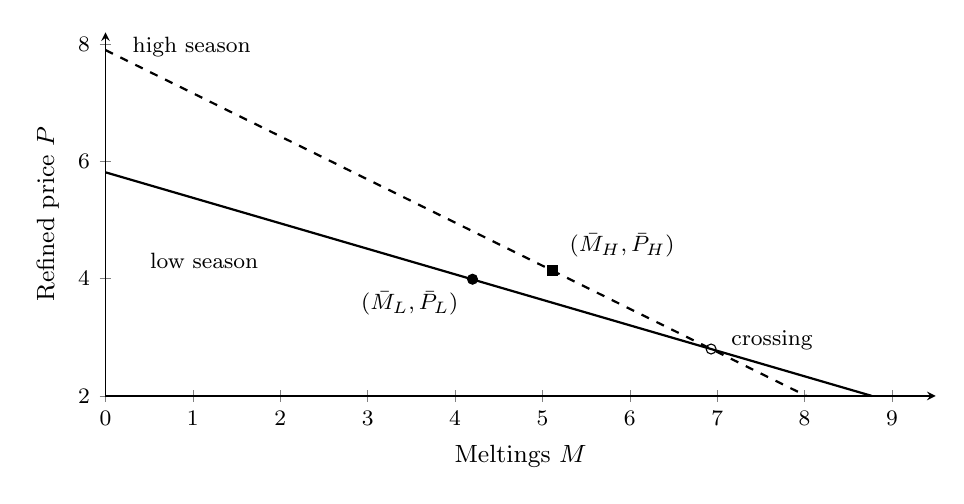
\begin{tikzpicture}
\begin{axis}[
  width=\linewidth, height=6.2cm,
  xmin=0, xmax=9.5, ymin=2, ymax=8.2,
  axis lines=left,
  xlabel={Meltings $M$}, ylabel={Refined price $P$},
  xlabel style={font=\small}, ylabel style={font=\small},
  tick label style={font=\footnotesize},
  clip=false]
\addplot[thick, black, domain=0:8.77, samples=2] {5.813 - x/2.30};
\addplot[thick, black, dashed, domain=0:8.02, samples=2] {7.897 - x/1.36};
\addplot[only marks, mark=*, mark size=1.8pt] coordinates {(4.20,3.99)};
\addplot[only marks, mark=square*, mark size=1.8pt] coordinates {(5.11,4.14)};
\addplot[only marks, mark=o, mark size=1.8pt] coordinates {(6.93,2.80)};
\node[font=\footnotesize, anchor=north west] at (axis cs:0.4,4.6) {low season};
\node[font=\footnotesize, anchor=west] at (axis cs:0.2,7.95) {high season};
\node[font=\footnotesize, anchor=south west] at (axis cs:5.2,4.2) {$(\bar M_H, \bar P_H)$};
\node[font=\footnotesize, anchor=north east] at (axis cs:4.15,3.95) {$(\bar M_L, \bar P_L)$};
\node[font=\footnotesize, anchor=west] at (axis cs:7.05,2.95) {crossing};
\end{axis}
\end{tikzpicture}
\caption{Demand: $M = 13.37 - 2.30P$ (solid) and $M = 10.74 - 1.36P$ (dashed).}
\end{subfigure}\hfill
\begin{subfigure}[t]{0.48\textwidth}
\centering
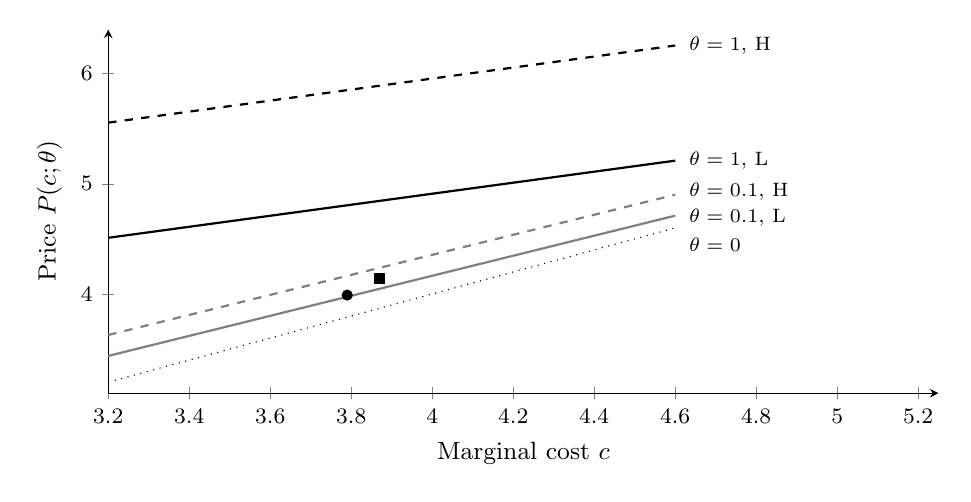
\begin{tikzpicture}
\begin{axis}[
  width=\linewidth, height=6.2cm,
  xmin=3.2, xmax=5.25, ymin=3.1, ymax=6.4,
  axis lines=left,
  xlabel={Marginal cost $c$}, ylabel={Price $P(c;\theta)$},
  xlabel style={font=\small}, ylabel style={font=\small},
  tick label style={font=\footnotesize},
  clip=false]
\addplot[thick, black, domain=3.2:4.6, samples=2] {(5.82 + x)/2};
\addplot[thick, black, dashed, domain=3.2:4.6, samples=2] {(7.91 + x)/2};
\addplot[thick, gray, domain=3.2:4.6, samples=2] {(0.582 + x)/1.1};
\addplot[thick, gray, dashed, domain=3.2:4.6, samples=2] {(0.791 + x)/1.1};
\addplot[thin, black, dotted, domain=3.2:4.6, samples=2] {x};
\addplot[only marks, mark=*, mark size=1.8pt] coordinates {(3.79,3.99)};
\addplot[only marks, mark=square*, mark size=1.8pt] coordinates {(3.87,4.14)};
\node[font=\scriptsize, anchor=west] at (axis cs:4.61,6.255) {$\theta = 1$, H};
\node[font=\scriptsize, anchor=west] at (axis cs:4.61,5.21) {$\theta = 1$, L};
\node[font=\scriptsize, anchor=west] at (axis cs:4.61,4.93) {$\theta = 0.1$, H};
\node[font=\scriptsize, anchor=west] at (axis cs:4.61,4.69) {$\theta = 0.1$, L};
\node[font=\scriptsize, anchor=west] at (axis cs:4.61,4.45) {$\theta = 0$};
\end{axis}
\end{tikzpicture}
\caption{Pricing rules $P(c;\theta) = \frac{\theta\alpha_s + c}{1 + \theta}$, low (solid) and high (dashed)
season.}
\end{subfigure}
\caption{The canning season rotates demand. Panel (a) shows the estimated linear demand curves, which cross at
$P = 2.80$, below all observed prices, and the season means. Panel (b) shows the implied pricing rules with
$\alpha_L = 5.82$ and $\alpha_H = 7.91$ (\cref{tab:03-gm-derived}). The monopoly price rises by
$\frac{\alpha_H - \alpha_L}{2} = 1.05$ in the high season at given cost, while competitive pricing does not
move. The markers are the season means of $(c_t, P_t)$ with $c_t = 0.26 + 1.075\,P^{\mathrm{raw}}_t$.
Constructed from \citet{GenesoveMullin1998}, Tables 2--4.}
\label{fig:03-gm-pricing-rules}
\end{figure}

\subsection{The direct measure of conduct}\label{sec:03-sugar-direct}

With demand in hand, the supply relation \eqref{eq:03-gm-supply} gives a pricing rule for every conduct
parameter.

\begin{proposition}[Pricing rules for the demand family]\label{prop:03-gm-pricing}
Let demand be \eqref{eq:03-gm-demand} and marginal cost $c$ be constant. The price that solves
\eqref{eq:03-gm-supply} is
\begin{equation}\label{eq:03-gm-pricing}
P(c;\theta) = \frac{\theta\alpha + \gamma c}{\gamma + \theta},
\qquad
P^M(c) \equiv P(c;1) = \frac{\alpha + \gamma c}{1 + \gamma}.
\end{equation}
In the log-linear case ($\alpha = 0$, $\gamma = -\varepsilon$) this is
$P(c;\theta) = \frac{\varepsilon}{\varepsilon - \theta}\,c$, and in the exponential limit it is
$P(c;\theta) = c + \frac{\theta}{\lambda}$. Pass-through is $\frac{\partial P}{\partial c} =
\frac{\gamma}{\gamma + \theta}$.
\end{proposition}

\begin{proof}
Since $P'(Q) = \frac{1}{Q'(P)}$, \cref{lem:03-gm-demand}(i) gives
\begin{equation*}
Q\,P'(Q) = \frac{Q(P)}{Q'(P)} = -\frac{\alpha - P}{\gamma}.
\end{equation*}
Substituting into \eqref{eq:03-gm-supply},
\begin{equation*}
P - \frac{\theta(\alpha - P)}{\gamma} = c
\;\Longleftrightarrow\;
\gamma P + \theta P = \gamma c + \theta\alpha
\;\Longleftrightarrow\;
P = \frac{\theta\alpha + \gamma c}{\gamma + \theta}.
\end{equation*}
Setting $\alpha = 0$ and $\gamma = -\varepsilon$ gives $P = \frac{-\varepsilon c}{\theta - \varepsilon} =
\frac{\varepsilon}{\varepsilon - \theta}c$. In the exponential limit, $\frac{\alpha - P}{\gamma} \to
\frac{1}{\lambda}$ by \cref{lem:03-gm-demand}(ii), so the supply relation reads $P - \frac{\theta}{\lambda} =
c$. Differentiating \eqref{eq:03-gm-pricing} in $c$ gives the pass-through.
\end{proof}

The pass-through formula agrees with \cref{prop:03-passthrough}. With flat marginal cost that proposition
gives $\rho = \frac{1}{1 + \theta(1 - \chi)}$, and $\chi = 1 - \frac{1}{\gamma}$ from
\cref{lem:03-gm-demand}(iii) yields $\rho = \frac{1}{1 + \frac{\theta}{\gamma}} = \frac{\gamma}{\gamma +
\theta}$. Two features matter below. The pricing rule is affine in cost with a slope that depends on $\theta$
and $\gamma$ only. Its intercept $\frac{\theta\alpha}{\gamma + \theta}$ moves with the season whenever
$\alpha$ does, and by more the larger is $\theta$. Under exponential demand the slope is one for every
$\theta$, so pass-through carries no information about conduct \citep{BulowPfleiderer1983}.

Monopoly requires an elastic demand at the monopoly price. At $P^M$, $\alpha - P^M = \frac{\gamma(\alpha -
c)}{1 + \gamma}$, so $\varepsilon(P^M) = \frac{\gamma P^M}{\alpha - P^M} = \frac{\alpha + \gamma c}{\alpha -
c}$. For $c > 0$ this exceeds one if and only if $\gamma > -1$ when $\alpha > c$, and $\gamma < -1$ when
$\alpha < c$ (WP p.~24). In the log-linear form, the high-season elasticity of 1.10 barely satisfies this
condition, and the implied monopoly price is enormous.

\Cref{tab:03-gm-derived} reports the implied pricing rules, the elasticities at the full-sample mean, and the
direct conduct measure.

\begin{table}[htbp]
\centering
\caption{Demand for refined sugar: derived estimates and the direct measure of conduct}\label{tab:03-gm-derived}
\small
\begin{tabular}{@{}lccccc@{}}
\toprule
 & (1) Quadratic & (2) Linear & (3) Log-linear & (4) Exponential & (5) Lerner\\
\midrule
$P^M(c)$, low season & $2.57 + 0.67c$ & $2.91 + 0.5c$ & $1.97c$ & $1.89 + c$ & \\
$P^M(c)$, high season & $3.96 + 0.67c$ & $3.96 + 0.5c$ & $10.1c$ & $3.85 + c$ & \\
\addlinespace
$P(c;\theta)$, low season & $\frac{7.72\theta + 2c}{2 + \theta}$ & $\frac{5.82\theta + c}{1 + \theta}$ &
 $\frac{2.03}{2.03 - \theta}c$ & $1.89\theta + c$ & \\[4pt]
$P(c;\theta)$, high season & $\frac{11.88\theta + 2c}{2 + \theta}$ & $\frac{7.91\theta + c}{1 + \theta}$ &
 $\frac{1.10}{1.10 - \theta}c$ & $3.85\theta + c$ & \\
\addlinespace
\multicolumn{6}{@{}l}{\textit{Elasticity $\varepsilon$ at the full-sample mean}}\\
Low season & 2.18 & 2.24 & 2.03 & 2.13 & \\
High season & 1.03 & 1.04 & 1.10 & 1.05 & \\
\addlinespace
\multicolumn{5}{@{}l}{\textit{Adjusted Lerner index $L_\varepsilon$}} & \textit{Unadjusted}\\
Mean & 0.099 & 0.107 & 0.095 & 0.097 & 0.054\\
Standard deviation & 0.097 & 0.118 & 0.083 & 0.089 & 0.045\\
Standard error & 0.024 & 0.028 & 0.021 & 0.022 & 0.0046\\
\bottomrule
\end{tabular}

\smallskip
\begin{minipage}{0.92\textwidth}\footnotesize
Notes: Reproduced from \citet{GenesoveMullin1998}, Table 4, which combines WP Tables 7 and 8. $L_\varepsilon =
\varepsilon\,\frac{P - c}{P}$ with $c = 0.26 + 1.075\,P^{\mathrm{raw}}$, computed quarter by quarter. The
standard errors account for the estimation of demand (WP Table 8, column 4). Standard errors that ignore it
are 0.010, 0.012, 0.008 and 0.009 (WP Table 8, column 3). WP Table 7 prints $7.88\theta$ in the high-season
linear rule.
\end{minipage}
\end{table}

\casehead{Checking the derived estimates}
Every entry follows from \cref{tab:03-gm-demand} and \cref{prop:03-gm-pricing}. In the quadratic form,
$P^M = \frac{7.72}{3} + \frac{2}{3}c = 2.57 + 0.67c$, and the high-season intercept is $\frac{11.88}{3} =
3.96$. In the linear form the choke prices are $\alpha_L = \frac{13.37}{2.30} = 5.81$ and $\alpha_H =
\frac{10.74}{1.36} = 7.90$, so $P^M = \frac{\alpha_s}{2} + \frac{c}{2}$ has intercepts 2.91 and 3.95. The
printed 5.82, 7.91 and 3.96 reflect unrounded coefficients. In the exponential form, $\frac{1}{0.53} = 1.89$
and $\frac{1}{0.26} = 3.85$. In the log-linear form, the monopoly markup factor
$\frac{\varepsilon}{\varepsilon - 1}$ equals $\frac{2.03}{1.03} = 1.97$ in the low season. In the high
season it equals $\frac{1.10}{0.10} = 11.0$ at $\varepsilon_H = 1.10$. The printed 10.1 corresponds to
$\varepsilon_H = \frac{10.1}{9.1} = 1.11$. Rounding cannot reconcile the two. Every elasticity in $[1.095,
1.105)$, which rounds to 1.10, gives a factor between 10.52 and 11.53. The published table is thus inconsistent
with its own elasticity, and the source does not explain why. The digits of 11.0 may have been transposed. We
reproduce the printed 10.1, which gives the high-season monopoly price of about 39 below. The factor 11.0 would
give about 43. The elasticities at $\bar P = 4.03$ follow from \cref{lem:03-gm-demand}(i). For example,
$\frac{2 \times 4.03}{7.72 - 4.03} = 2.18$ and $\frac{2 \times 4.03}{11.88 - 4.03} = 1.03$ for the quadratic,
$0.53 \times 4.03 = 2.14$ (2.13 in the table, from unrounded coefficients) and $0.26 \times 4.03 = 1.05$ for the
exponential.

\casehead{Observed prices are far below monopoly}
At the low-season means, marginal cost is $c = 0.26 + 1.075 \times 3.28 = 3.79$. The linear monopoly price
is then $2.91 + 0.5 \times 3.79 = 4.80$, against an observed mean of 3.99. In the high season, $c = 0.26 +
1.075 \times 3.36 = 3.87$ and $P^M = 3.96 + 0.5 \times 3.87 = 5.90$, against 4.14. The quadratic form puts
the monopoly prices at 5.10 and 6.54, the exponential form at 5.68 and 7.72, and the log-linear form at 7.47
and about 39. Whatever the demand form, the industry priced far below the monopoly level (WP p.~27). Panel (b) of
\cref{fig:03-gm-pricing-rules} shows the gap.

\casehead{The direct measure}
The first estimation method uses everything. Marginal cost is \eqref{eq:03-gm-direct-cost}, the elasticity
comes from the season's demand curve evaluated at the quarter's price, and conduct is computed quarter by
quarter:
\begin{equation}\label{eq:03-gm-direct}
L_{\varepsilon t} = \varepsilon_{s(t)}(P_t)\,\frac{P_t - c_t}{P_t} = \frac{P_t - c_t}{m_t},
\qquad m_t = \frac{\alpha_{s(t)} - P_t}{\gamma_{s(t)}} .
\end{equation}
The second expression uses \cref{lem:03-gm-demand}(i): conduct is the price-cost margin divided by the
markup term $m_t = \frac{Q_t}{\lvert Q'(P_t)\rvert}$ of \cref{sec:03-corts}. The direct measure is a
function of data and of the estimated demand parameters. Its standard error must reflect the second source
of noise. Genesove and Mullin stack the demand moment conditions with the moment
$\frac{1}{n}\sum_t \left(L_{\varepsilon t} - \bar L_\varepsilon\right) = 0$ and compute the usual GMM
variance for the mean $\bar L_\varepsilon$ (WP p.~31, fn.~45). Accounting for estimated demand more than
doubles the standard errors.

\casehead{Results}
The mean adjusted Lerner index lies between 0.095 and 0.107 across the four demand forms
(\cref{tab:03-gm-derived}). Genesove and Mullin take $\theta = 0.10$ as their direct measure. This is the
conduct of a static symmetric Cournot oligopoly with ten firms. Both perfect competition and monopoly are
rejected: the mean is about four standard errors above zero and far below one. The unadjusted Lerner index
of 0.054 says that price exceeded marginal cost by only 5 percent. With demand elasticities near two, even
this small margin corresponds to a conduct parameter of 0.10. With the lower bound $c_0 = 0.16$, the mean index
rises to 0.14 (log-linear and exponential), 0.15 (quadratic) and 0.16 (linear). The value $0.15$ corresponds
to a symmetric Cournot oligopoly with about seven firms, so the conclusions do not change (WP p.~37).

\begin{figure}[!htb]
\centering
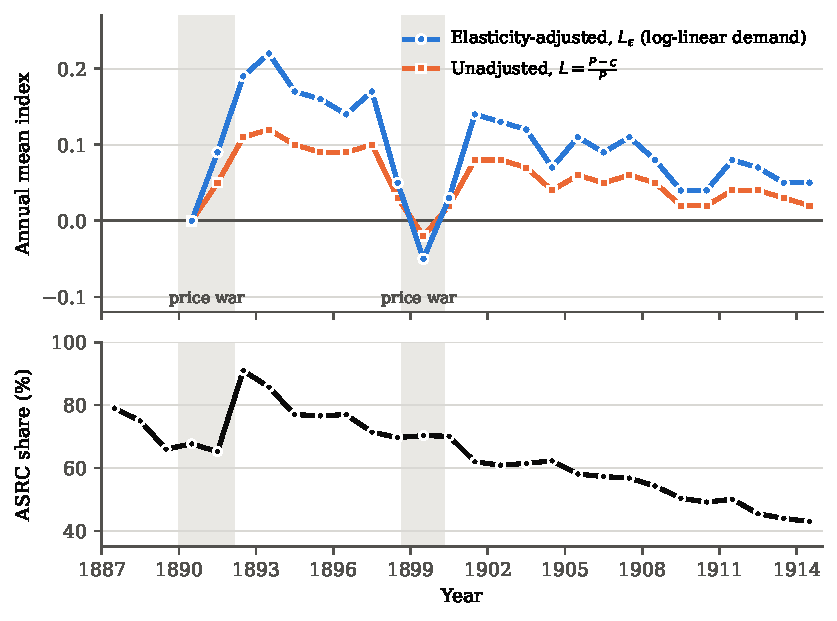
\includegraphics[width=0.86\textwidth]{figures/ch03/gm_lerner_time.pdf}
\caption{Annual means of the unadjusted Lerner index $\frac{P - c}{P}$ and of the elasticity-adjusted index
$L_\varepsilon$ (log-linear demand), top, and the market share of the American Sugar Refining Company,
bottom. Shaded bands mark the two post-entry price wars (January 1890 to February 1892 and September 1898 to
April 1900). Redrawn from \citet{GenesoveMullin1995}, WP Table 9.}
\label{fig:03-gm-lerner-time}
\end{figure}

\casehead{Conduct over time}
\Cref{fig:03-gm-lerner-time} plots the annual means of WP Table 9. Conduct follows structure. The adjusted
index is zero in 1890 during the Spreckels war. It rises to between 0.14 and 0.22 in 1892--1897, after ASRC
had consolidated 91 percent of the market. It collapses again in the Arbuckle war, to $-0.05$ in 1899,
which means pricing below the measured marginal cost. Willett and Gray themselves reported in October 1898
that refiners were selling at ``an actual loss'' (WP p.~33, fn.~47). After 1900 the index drifts down from
0.14 to about 0.05 as ASRC's share falls toward 43 percent. Across the twenty years outside the price wars (excluding 1890, 1891 and 1898--1900),
the correlation between the annual adjusted index and ASRC's share is 0.92 (our computation from WP Table 9).
The averages over 1890--1914 are 0.09 for the adjusted index, 0.05 for the unadjusted index and 63.1 percent
for ASRC's share.

\begin{table}[htbp]
\centering
\caption{Seasonality of the direct conduct measure}\label{tab:03-gm-seasonality}
\small
\begin{tabular}{@{}lcccccccc@{}}
\toprule
 & \multicolumn{2}{c}{Quarter I} & \multicolumn{2}{c}{Quarter II} & \multicolumn{2}{c}{Quarter III (high)} &
 \multicolumn{2}{c}{Quarter IV}\\
\cmidrule(lr){2-3}\cmidrule(lr){4-5}\cmidrule(lr){6-7}\cmidrule(l){8-9}
 & Mean & S.D. & Mean & S.D. & Mean & S.D. & Mean & S.D.\\
\midrule
Unadjusted $L$ & 0.048 & 0.042 & 0.065 & 0.042 & 0.064 & 0.047 & 0.038 & 0.047\\
$L_\varepsilon$, quadratic & 0.096 & 0.091 & 0.142 & 0.104 & 0.071 & 0.057 & 0.083 & 0.117\\
$L_\varepsilon$, linear & 0.102 & 0.106 & 0.162 & 0.138 & 0.075 & 0.063 & 0.086 & 0.134\\
$L_\varepsilon$, log-linear & 0.097 & 0.085 & 0.132 & 0.085 & 0.071 & 0.051 & 0.078 & 0.096\\
$L_\varepsilon$, exponential & 0.097 & 0.087 & 0.136 & 0.092 & 0.071 & 0.055 & 0.081 & 0.106\\
\bottomrule
\end{tabular}

\smallskip
\begin{minipage}{0.92\textwidth}\footnotesize
Notes: Reproduced from \citet{GenesoveMullin1995}, WP Table 10. Means and standard deviations across
quarters of the same type.
\end{minipage}
\end{table}

\casehead{Conduct over the year}
\Cref{tab:03-gm-seasonality} shows that conduct also varies within the year. It is least competitive in the
second quarter and most competitive in the third, the high season. This pattern fits dynamic oligopoly models
in which the expectation of better demand ahead helps collusion and the expectation of worse demand harms it
\citep{RotembergSaloner1986,HaltiwangerHarrington1991}. Genesove and Mullin note a caveat. The unadjusted
index is equal in the second and third quarters, so the pattern may be an artifact of attaching the
inelastic high-season demand to the third quarter alone (WP pp.~33--34). Either way, conduct that varies
systematically with a demand shifter contradicts the assumption of the NEIO method that $\theta$ is
uncorrelated with the instruments. Genesove and Mullin argue that the proper test of a method is its success in
doing what it is meant to do, whatever the truth of its assumptions (WP p.~34). The next subsection shows that this
seasonal pattern explains much of what the NEIO estimator finds.

The low level of the index, relative to the industry's concentration, has a natural explanation. Pricing was
constrained by the threat of domestic entry and of foreign imports (WP p.~34). The price wars of 1890 and
1898--1900 show that the entry threat was not idle.

\subsection{Estimating conduct with cost treated as unknown}\label{sec:03-sugar-neio}

We now put ourselves in the position of an NEIO researcher who observes prices, quantities, the raw sugar
price and the instruments, but does not know $c_0$, $k$ or both.

\casehead{The pricing equation}
Substituting \eqref{eq:03-gm-cost} into \eqref{eq:03-gm-pricing} gives the reduced-form pricing equation
(WP eq.~12)
\begin{equation}\label{eq:03-gm-reduced}
P_t = \frac{\alpha_{s}\theta + c_0\gamma_{s}}{\gamma_{s} + \theta}
 + \frac{\gamma_{s}}{\gamma_{s} + \theta}\,k\,P^{\mathrm{raw}}_t + u_t ,
\qquad s = s(t),
\end{equation}
where $u_t$ is a pricing error from unobserved cost or conduct shocks. In the exponential case the equation
is $P_t = \frac{\theta}{\lambda_s} + c_0 + kP^{\mathrm{raw}}_t + u_t$ (WP p.~34, fn.~49). Multiplying
\eqref{eq:03-gm-reduced} by $\gamma_s + \theta$ gives the moment condition that Genesove and Mullin estimate
(WP eq.~13):
\begin{equation}\label{eq:03-gm-moment}
\E\Big[\big\{(\gamma_s + \theta)P_t - \alpha_s\theta - c_0\gamma_s - \gamma_s k P^{\mathrm{raw}}_t\big\}\,z_t\Big]
= 0 .
\end{equation}
The demand parameters $(\alpha_s, \gamma_s)$ are fixed at their estimates in \cref{tab:03-gm-demand}. The
unknowns are $\theta$ and whichever cost parameters the researcher does not know.

The raw price must be instrumented. Whether $u_t$ is a cost shock or a conduct shock, a positive $u_t$ raises
the refined price and lowers the quantity of refined sugar demanded. Refiners then demand less raw sugar,
which lowers the raw price. The pricing error is therefore negatively correlated with $P^{\mathrm{raw}}_t$ (WP
p.~34). Log Cuban imports again serve as the excluded cost shifter.

\casehead{The information hierarchy}
Genesove and Mullin organize the comparison by what the researcher knows about cost (WP p.~35).
\begin{enumerate}[label=(\Roman*)]
\item Neither $c_0$ nor $k$ is known. The unknowns are $(\theta, c_0, k)$, and the instruments are
$z_t = (1, H_t, \ln\mathit{CUBA}_t)$.
\item The input coefficient $k = 1.075$ is known, and $c_0$ is not. The unknowns are $(\theta, c_0)$, and the
instruments are $z_t = (1, H_t)$. This is the position of the cigarette studies of \citet{Sumner1981},
\citet{Sullivan1985} and \citet{AshenfelterSullivan1987} (\cref{sec:03-sumner}). In those studies an excise
tax enters marginal cost with a known coefficient of one.
\item Both $c_0 = 0.26$ and $k = 1.075$ are known. Then $\theta$ is observed directly, as in
\eqref{eq:03-gm-direct}.
\end{enumerate}
The fourth combination, $c_0$ known and $k$ unknown, is implausible in this industry and is not explored. In
both (I) and (II) the number of instruments equals the number of unknowns, so the nonlinear instrumental
variables (NLIV) estimator solves the sample analogue of \eqref{eq:03-gm-moment} exactly. Estimating demand
first and the pricing equation second is the two-step method. Stacking the demand moments and
\eqref{eq:03-gm-moment} in a single GMM problem is the joint version of the same estimator.

\casehead{Standard errors with estimated demand}
The two-step estimator inherits the noise in the demand estimates. Let $b = (\theta, c_0, k)^\T$, let $a$ be
the demand parameters with $\sqrt{n}(\hat a - a_0) \to N(0, W_1)$, and let $\bar g_n(b, a)$ be the sample
analogue of \eqref{eq:03-gm-moment}. A mean-value expansion of $\bar g_n(\hat b, \hat a) = 0$ around
$(b_0, a_0)$ gives
\begin{equation*}
0 = \bar g_n(b_0, a_0) + D\,(\hat b - b_0) + C\,(\hat a - a_0) + o_p\!\left(n^{-\frac{1}{2}}\right),
\qquad D = \E\left[\frac{\partial g}{\partial b^\T}\right],\;\; C = \E\left[\frac{\partial g}{\partial a^\T}\right].
\end{equation*}
Solving for $\hat b - b_0$,
\begin{equation*}
\sqrt{n}\,(\hat b - b_0) = -D^{-1}\sqrt{n}\,\bar g_n(b_0, a_0) - D^{-1}C\,\sqrt{n}\,(\hat a - a_0) + o_p(1).
\end{equation*}
If the pricing moments and the demand estimates are asymptotically uncorrelated, the asymptotic variance is
\begin{equation}\label{eq:03-gm-variance}
\operatorname{Avar}(\hat b) = W_2 + D^{-1} C\, W_1\, C^\T \left(D^{-1}\right)^\T,
\qquad W_2 = D^{-1} S \left(D^{-1}\right)^\T ,
\end{equation}
where $S$ is the long-run variance of the pricing moments. Genesove and Mullin estimate $S$ and $W_1$ by
Newey-West with four lags (WP p.~36). The zero-correlation assumption fits their interpretation: demand errors
are proportional shifts that do not move the pricing rule. Without it, the joint GMM estimator delivers
correct standard errors directly (\cref{app:econometrics}).

\begin{table}[htbp]
\centering
\caption{NLIV estimates of conduct and cost parameters}\label{tab:03-gm-nliv}
\small
\setlength{\tabcolsep}{4.5pt}
\begin{tabular}{@{}lccccccccc@{}}
\toprule
 & \multicolumn{2}{c}{Quadratic} & \multicolumn{2}{c}{Linear} & \multicolumn{2}{c}{Log-linear} &
 \multicolumn{2}{c}{Exponential} & Direct\\
\cmidrule(lr){2-3}\cmidrule(lr){4-5}\cmidrule(lr){6-7}\cmidrule(lr){8-9}\cmidrule(l){10-10}
 & (1) & (2) & (3) & (4) & (5) & (6) & (7) & (8) & (9)\\
\midrule
$\hat\theta$ & 0.037 & 0.035 & 0.038 & 0.037 & 0.045 & 0.040 & 0.041 & 0.037 & 0.10\\
 & (0.024) & (0.024) & (0.024) & (0.024) & (0.028) & (0.026) & (0.026) & (0.025) & \\
$\hat c_0$ & 0.529 & 0.393 & 0.465 & 0.39 & 0.760 & 0.381 & 0.700 & 0.389 & 0.26\\
 & (0.272) & (0.062) & (0.285) & (0.061) & (0.262) & (0.070) & (0.279) & (0.065) & \\
$\hat k$ & 1.033 & & 1.052 & & 0.956 & & 0.978 & & 1.075\\
 & (0.082) & & (0.085) & & (0.081) & & (0.083) & & \\
\bottomrule
\end{tabular}

\smallskip
\begin{minipage}{0.92\textwidth}\footnotesize
Notes: Reproduced from \citet{GenesoveMullin1995}, WP Table 11. Columns (1), (3), (5) and (7) estimate
$(\theta, c_0, k)$ with instruments $(1, H_t, \ln\mathit{CUBA}_t)$. Columns (2), (4), (6) and (8) impose $k =
1.075$ and use $(1, H_t)$. Demand parameters from \cref{tab:03-gm-demand}. Newey-West standard errors (four
lags), corrected for estimated demand, in parentheses. Column (9) is the direct measure. $N = 97$.
\end{minipage}
\end{table}

\casehead{Results}
\Cref{tab:03-gm-nliv} reports the estimates. Genesove and Mullin draw four conclusions (WP pp.~36--37).
First, the NLIV estimate of $\theta$ is close to the direct measure. It lies between 0.035 and 0.045 in all
eight specifications. Monopoly is rejected everywhere, as is any $\theta$ above 0.11. Perfect competition
cannot be rejected: the $t$ ratios are between 1.46 and 1.61. The estimates are below the direct measure in
every case. The upper limits of the 95 percent confidence intervals run from 0.082 to 0.100 (our computation),
so the direct value of 0.10 sits at or just beyond their edge. Second, the estimates are robust to the form
of demand. This answers the common complaint that conduct estimates hinge on functional form. Third, the cost
parameters are recovered less well. The coefficient $k$ is underestimated in all four forms, although
$k = 1.075$ is never rejected. The parameter $c_0$ is overestimated, by 50 cents in the log-linear case (0.760
against 0.26). Fourth, knowing $k$ hardly changes $\hat\theta$. It sharpens the estimate of $c_0$, which falls to
0.38--0.39 with standard errors near 0.06. Because $c_0$ does not enter the NLIV estimator, setting $c_0 =
0.16$ leaves \cref{tab:03-gm-nliv} unchanged and moves only the benchmark, from 0.10 to about 0.15.

\casehead{What identifies $\theta$: the seasonal shift}
Why does the method deliver 0.04? In the quadratic, linear and exponential forms only the intercept of
\eqref{eq:03-gm-reduced} differs across seasons. The equation can then be written as a linear regression,
\begin{equation}\label{eq:03-gm-linear-rf}
P_t = \pi_0 + \pi_1 H_t + \pi_2 P^{\mathrm{raw}}_t + u_t .
\end{equation}
For the linear and quadratic forms, with $\gamma$ common to both seasons,
\begin{equation*}
\pi_0 = \frac{\theta\alpha_L + \gamma c_0}{\gamma + \theta},
\qquad
\pi_1 = \frac{\theta\,(\alpha_H - \alpha_L)}{\gamma + \theta},
\qquad
\pi_2 = \frac{\gamma k}{\gamma + \theta}.
\end{equation*}
For the exponential form, $\pi_0 = \frac{\theta}{\lambda_L} + c_0$, $\pi_1 = \theta\left(\frac{1}{\lambda_H} -
\frac{1}{\lambda_L}\right)$ and $\pi_2 = k$. In each case the map from $(\theta, c_0, k)$ to $(\pi_0, \pi_1,
\pi_2)$ is one to one. For the linear and quadratic forms, inverting it gives
\begin{equation}\label{eq:03-gm-inversion}
\theta = \frac{\gamma\,\pi_1}{(\alpha_H - \alpha_L) - \pi_1},
\qquad
k = \frac{\gamma + \theta}{\gamma}\,\pi_2,
\qquad
c_0 = \frac{(\gamma + \theta)\pi_0 - \theta\alpha_L}{\gamma}.
\end{equation}
The conduct parameter is identified only through $\pi_1$, the seasonal shift of the pricing rule at a given
raw price. If the season changed only the scale $\beta$, so that $\alpha_H = \alpha_L$, then $\pi_1 = 0$ for
every $\theta$ and conduct would not be identified. A seasonal change in $\alpha$ suffices, even a parallel
shift of linear demand. Identification therefore rests on the restriction that marginal cost is constant in
output (\cref{sec:03-other-routes}). The general rotation argument of \cref{prop:03-rotation,prop:03-lau} is
needed only when the slope of marginal cost is unknown. At $\theta = 1$,
$\pi_1$ equals the seasonal shift of the monopoly price, $\frac{\alpha_H - \alpha_L}{1 + \gamma}$. The
estimator thus compares the observed seasonal price shift with the shift that a monopolist would make.

\begin{table}[htbp]
\centering
\caption{Linear pricing equations for refined sugar}\label{tab:03-gm-reduced}
\small
\begin{tabular}{@{}lcccccc@{}}
\toprule
 & (1) & (2) & (3) & (4) & (5) & (6)\\
 & IV & IV & IV & OLS & OLS & OLS\\
\midrule
Raw price & 1.02 & 0.93 & 1.01 & 0.99 & 0.98 & 0.99\\
 & (0.09) & (0.09) & (0.08) & (0.05) & (0.05) & (0.05)\\
High season $\times$ raw price & & 0.31 & & & 0.04 & \\
 & & (0.11) & & & (0.07) & \\
High season & & $-0.97$ & 0.08 & & $-0.07$ & 0.08\\
 & & (0.38) & (0.03) & & (0.22) & (0.03)\\
Constant & 0.67 & 0.94 & 0.66 & 0.75 & 0.77 & 0.74\\
 & (0.28) & (0.28) & (0.26) & (0.16) & (0.16) & (0.16)\\
$\chi^2_{(2)}$ test & & 21.67 & & & 6.66 & \\
\bottomrule
\end{tabular}

\smallskip
\begin{minipage}{0.92\textwidth}\footnotesize
Notes: Reproduced from \citet{GenesoveMullin1995}, WP Table 12. Dependent variable: refined price, $N = 97$.
Instruments in columns (1) and (2): high season, log Cuban imports and their interaction. The $\chi^2_{(2)}$
statistic tests that the coefficients on high season and its interaction with the raw price are both zero.
\end{minipage}
\end{table}

Column (3) of \cref{tab:03-gm-reduced} estimates \eqref{eq:03-gm-linear-rf} by instrumental variables. The
refined price rises by only 8 cents in the high season at a given raw price. The demand estimates imply
much larger shifts of the monopoly price: $\frac{\alpha_H - \alpha_L}{2} = 1.05$ for linear demand and
$\frac{1}{\lambda_H} - \frac{1}{\lambda_L} = 3.85 - 1.89 = 1.96$ for exponential demand. Under exponential
demand the intercept is $\frac{\theta}{\lambda_s} + c_0$, so
\begin{equation*}
\hat\theta \approx \frac{0.08}{1.96} \approx 0.04
\end{equation*}
(WP p.~38). Under linear demand, \eqref{eq:03-gm-inversion} with $\gamma = 1$ and $\alpha_H - \alpha_L =
7.91 - 5.82 = 2.09$ gives
\begin{equation*}
\theta = \frac{0.08}{2.09 - 0.08} = 0.040,
\quad
k = 1.040 \times 1.01 = 1.050,
\quad
c_0 = 1.040 \times 0.66 - 0.040 \times 5.82 = 0.455 .
\end{equation*}
These reproduce column (3) of \cref{tab:03-gm-nliv}, $(0.038, 0.465, 1.052)$, up to rounding. The quadratic form
gives $(0.039, 0.52, 1.03)$ against $(0.037, 0.529, 1.033)$. The same arithmetic explains the cost
estimates. The raw-price coefficient of 1.01 forces $k$ below 1.075, because the slope $\frac{\gamma
k}{\gamma + \theta}$ is close to $k$ when $\theta$ is small. With $\theta$ understated, $c_0$ must absorb
the remaining margin between the refined and raw prices, so $c_0$ is overstated (WP p.~38).

\casehead{A closed form when $k$ is known}
When $k$ is known, the estimator has an explicit form that links it to the direct measure. Divide the
expression in braces in \eqref{eq:03-gm-moment} by $\gamma_s$ and use \cref{lem:03-gm-demand}(i):
\begin{equation*}
\frac{(\gamma_s + \theta)P_t - \alpha_s\theta - c_0\gamma_s - \gamma_s k P^{\mathrm{raw}}_t}{\gamma_s}
= \big(P_t - kP^{\mathrm{raw}}_t\big) - c_0 - \theta\,\frac{\alpha_s - P_t}{\gamma_s}
= G_t - c_0 - \theta\, m_t .
\end{equation*}
The pricing equation thus says that the proper margin equals non-sugar cost plus conduct times the markup
term. This holds in all four forms, and in the exponential form $m_t = \frac{1}{\lambda_s}$.

\begin{proposition}[The NLIV estimator with known $k$]\label{prop:03-gm-wald}
Suppose $k$ is known, the instruments are $(1, H_t)$, and demand is quadratic, linear or exponential. Let $\bar G_s$ and $\bar m_s$ be the season means of the proper
margin and of the markup term. Then
\begin{equation}\label{eq:03-gm-wald}
\hat\theta = \frac{\bar G_H - \bar G_L}{\bar m_H - \bar m_L},
\qquad
\hat c_0 = \bar G_L - \hat\theta\,\bar m_L .
\end{equation}
If the true marginal cost is \eqref{eq:03-gm-cost} and $\theta_t$ denotes true conduct, then
\begin{equation}\label{eq:03-gm-corts}
\hat\theta = \frac{\overline{(\theta m)}_H - \overline{(\theta m)}_L}{\bar m_H - \bar m_L},
\end{equation}
where $\overline{(\theta m)}_s$ is the season mean of $\theta_t m_t$.
\end{proposition}

\begin{proof}
In the quadratic and linear forms $\gamma$ is common to both seasons, so multiplying each moment by the
constant $\frac{1}{\gamma}$ does not change the solution. In the exponential form the moment is
$G_t - c_0 - \theta m_t$ to begin with. The sample moments with instruments $1$ and $H_t$ are
$\sum_t (G_t - c_0 - \theta m_t) = 0$ and $\sum_t H_t(G_t - c_0 - \theta m_t) = 0$. Their difference is the
sum over low-season quarters, so the two conditions are equivalent to
$\bar G_s = c_0 + \theta\,\bar m_s$ for $s = L, H$. Subtracting the low-season equation from the high-season
equation gives $\hat\theta$, and the low-season equation then gives $\hat c_0$. For the second part, the
definition of true conduct in \eqref{eq:03-gm-direct} gives $P_t - c_t = \theta_t m_t$, so $G_t = c_0 +
\theta_t m_t$ by \eqref{eq:03-gm-proper-margin}. Taking season means and substituting into
\eqref{eq:03-gm-wald} gives \eqref{eq:03-gm-corts}.
\end{proof}

The estimator is a Wald ratio. It divides the seasonal change in the proper margin by the seasonal change in
the markup term predicted by demand. With the published season means, $\bar G_H - \bar G_L = 0.53 - 0.46 =
0.07$ (\cref{tab:03-gm-stats}). In the linear form, $\bar m_s = \alpha_s - \bar P_s$, so $\bar m_H - \bar m_L
= 2.09 - 0.15 = 1.94$. In the exponential form, $\bar m_H - \bar m_L = 1.96$. Hence
\begin{align*}
\text{linear:}\quad & \hat\theta = \frac{0.07}{1.94} = 0.036, &
\hat c_0 &= 0.46 - 0.036 \times 1.83 = 0.39,\\
\text{exponential:}\quad & \hat\theta = \frac{0.07}{1.96} = 0.036, &
\hat c_0 &= 0.46 - 0.036 \times 1.89 = 0.39 .
\end{align*}
Columns (4) and (8) of \cref{tab:03-gm-nliv} report $(0.037, 0.39)$ and $(0.037, 0.389)$. The rounding of the
season means to two decimals limits the precision of this check to about $\pm 0.005$ in $\hat\theta$. The
formula also explains the robustness across forms. Each form predicts nearly the same seasonal change in
the markup term at observed prices, between 1.8 dollars (log-linear, $\frac{4.14}{1.10} - \frac{3.99}{2.03}$
at the season means) and 2.0 dollars (quadratic). The four forms differ greatly far from the
data, as their monopoly prices show, but they agree near it.

\casehead{The Corts critique in the sugar data}
Equation \eqref{eq:03-gm-corts} is the IV estimand of \cref{prop:03-corts} with the season indicator as the
instrument. It equals average conduct only if conduct does not differ between seasons. In the exponential
form the markup term is constant within a season, $m_t = \frac{1}{\lambda_s}$. Writing $\bar\theta_s$ for the
season mean of the direct measure, \eqref{eq:03-gm-corts} becomes
\begin{equation*}
\hat\theta
= \frac{\frac{\bar\theta_H}{\lambda_H} - \frac{\bar\theta_L}{\lambda_L}}{\frac{1}{\lambda_H} - \frac{1}{\lambda_L}}
= \frac{3.85\,\bar\theta_H - 1.89\,\bar\theta_L}{1.96}
= \bar\theta_H - 0.96\,\big(\bar\theta_L - \bar\theta_H\big).
\end{equation*}
\Cref{tab:03-gm-seasonality} gives $\bar\theta_H = 0.071$ for the exponential form. The low-season quarters
average about 0.105, weighting quarters I, II and IV by their numbers of observations. Then $\hat\theta = 0.071 - 0.96 \times 0.034 = 0.038$, essentially the reported
0.037. Implied non-sugar cost is $0.26 + (0.105 - 0.038) \times 1.89 = 0.39$, the reported 0.389. The
NLIV estimate lies below even the high-season conduct, because conduct is lower exactly when the rotator is
on. If conduct had stayed at its mean of about 0.10 throughout, the proper margin would have risen by
$0.10 \times 1.96 = 0.20$ in the high season. It rose by 0.07. The understatement of $\theta$ and the
overstatement of $c_0$ both reflect the mechanism of \citet{Corts1999}. The estimator measures the response of
the margin to the rotation, and here that response understates the level of conduct.\footnote{This decomposition is ours. Genesove and Mullin
report the seasonal pattern and the NLIV estimates separately, and attribute the pattern to dynamic
oligopoly (WP pp.~33--34).}

\casehead{The log-linear form}
Under log-linear demand the slope of the pricing rule, $\frac{\varepsilon_s}{\varepsilon_s - \theta}k$,
differs by season, so the linear reparameterization needs an interaction, column (2) of
\cref{tab:03-gm-reduced}. The lower high-season elasticity predicts a steeper pricing rule in the high
season, and the interaction is positive and significant (0.31). The intercept $\frac{\varepsilon_s c_0}
{\varepsilon_s - \theta}$ should also be higher in the high season, yet the high-season coefficient is
$-0.97$. Using the slopes alone gives $\theta = 0.46$. With $r = \frac{0.93 + 0.31}{0.93}$ the ratio of the
slopes, the condition $\frac{\varepsilon_H(\varepsilon_L - \theta)}{\varepsilon_L(\varepsilon_H - \theta)} = r$
solves for $\theta = 0.463$. Using the intercepts alone gives the nonsensical 2.09 (WP p.~39). The NLIV
estimator forces the ratio of intercept to slope to be the same in both seasons, $\frac{c_0}{k}$, and so
returns estimates close to the other forms. Its implied pricing rules are $P = 0.777 + 0.978\,P^{\mathrm{raw}}$
in the low season and $P = 0.792 + 0.997\,P^{\mathrm{raw}}$ in the high season (our computation from column
(5)).\footnote{WP p.~39, fn.~52, prints $0.793 + 0.997\,P^{\mathrm{raw}}$ for the low season and $0.777 + 0.977\,
P^{\mathrm{raw}}$ for the high season. The factor $\frac{\varepsilon_s}{\varepsilon_s - \theta}$ is larger for the
smaller high-season elasticity, so the steeper rule must belong to the high season. The labels in the footnote
appear to be interchanged.} None of the four forms is consistent with the unrestricted estimates of column (2)
(WP p.~39). The other three forms require equal slopes in the two seasons, a single restriction on the
interaction. Its $t$ ratio is $\frac{0.31}{0.11} = 2.8$, a Wald statistic of about 7.9, so equal slopes are
rejected at the 1 percent level. The $\chi^2_{(2)}$ statistic of 21.67 tests a different hypothesis, that
the seasonal intercept and the interaction are both zero. Genesove and Mullin describe the low-season slope of
0.93 as significantly below 1.075, which would contradict log-linear demand, under which price rises more than
one for one with cost. Its $t$ ratio is only $\frac{1.075 - 0.93}{0.09} = 1.61$. The gap is significant at
the one-sided 10 percent level, and not at the one-sided 5 percent level or at any conventional two-sided level.

\casehead{Ignoring the seasons}
Column (1) of \cref{tab:03-gm-reduced} drops all seasonal effects, as a researcher would who used the known
$k$ but ignored the rotation. The only remaining information on conduct is the slope of the pricing rule,
$\frac{\gamma k}{\gamma + \theta} = 1.02$. Solving,
\begin{equation*}
\theta = \gamma\left(\frac{1.075}{1.02} - 1\right) = 0.054\,\gamma .
\end{equation*}
The implied conduct is proportional to the assumed curvature. It equals 0.054 for linear demand and 0.108 for
quadratic demand (WP p.~39). Quadratic demand without seasons has choke price $\hat\alpha = 8.63$ (standard
error 1.17), and it also gives an excellent estimate of non-sugar cost, $\hat c_0 = 0.23$.\footnote{WP p.~39
prints the fitted curve as $\ln M = 7.37 + 2\ln(8.63 - P)$, with standard errors 0.50 and 1.17. The working
paper measures meltings in hundreds of thousands of long tons (WP p.~26), as in \cref{tab:03-gm-stats}. In
those units the printed intercept predicts meltings of about 34{,}000 at $P = 4$, against a sample mean of
4.43. The source does not say whether the intercept is a misprint or uses another unit. Only the choke price
enters the pricing equation, since $m_t = \frac{\alpha - P_t}{2}$.} The researcher
would have no way to know which answer is right. This is the curvature critique of pass-through tests in
\cref{sec:03-sumner} in another guise: the slope identifies conduct only given $\gamma$. With exponential
demand the slope is $k$ for every $\theta$, and $\theta$ and $c_0$ are not even separately identified
\citep{BulowPfleiderer1983}.

\begin{table}[htbp]
\centering
\caption{Cost estimates and predicted price changes under imposed behavioral models}\label{tab:03-gm-behavioral}
\small
\setlength{\tabcolsep}{4.2pt}
\begin{tabular}{@{}lccccccccc@{}}
\toprule
 & \multicolumn{2}{c}{Competition} & \multicolumn{2}{c}{Cournot I} & \multicolumn{2}{c}{Cournot II} &
 \multicolumn{2}{c}{Monopoly} & Direct\\
\cmidrule(lr){2-3}\cmidrule(lr){4-5}\cmidrule(lr){6-7}\cmidrule(lr){8-9}\cmidrule(l){10-10}
 & (1) & (2) & (3) & (4) & (5) & (6) & (7) & (8) & (9)\\
\midrule
$\hat c_0$ & 0.674 & 0.476 & 0.00 & 0.069 & 0.00 & 0.00 & 0.00 & 0.00 & 0.26\\
 & (0.281) & (0.034) & (0.239) & (0.071) & (0.922) & (0.400) & (1.65) & (0.563) & \\
$\hat k$ & 1.015 & & 1.096 & & 0.883 & & 0.529 & & 1.075\\
 & (0.087) & & (0.071) & & (0.253) & & (0.471) & & \\
\addlinespace
$\widehat{\Delta P}$ & 0.689 & 0.729 & 0.620 & 0.608 & 0.300 & 0.365 & 0.179 & 0.365 & 0.702\\
 & (0.059) & & (0.040) & & (0.086) & & (0.086) & & \\
\bottomrule
\end{tabular}

\smallskip
\begin{minipage}{0.92\textwidth}\footnotesize
Notes: Reproduced from \citet{GenesoveMullin1998}, Table 9. Linear demand estimated by season. Cost parameters
constrained to be nonnegative. Columns (1), (3), (5) and (7) estimate $k$ with a constant and log Cuban
imports as instruments. Columns (2), (4), (6) and (8), where $\hat k$ is blank, impose $k = 1.075$ and use a
constant only (p.~371, n.~30). In columns (1) to (8),
$\widehat{\Delta P}$ is the predicted rise in the refined price. The shock is the rise in the raw price by 68
cents per hundred pounds from the third quarter of 1896 to the third quarter of 1897. Column (9) reports the
realized rise (p.~374).
\end{minipage}
\end{table}

\casehead{Imposing a behavioral model}
The published article adds an exercise that shows what goes wrong when conduct is assumed (Table 9,
reproduced in \cref{tab:03-gm-behavioral}). The researcher fixes $\theta$ at the value implied by a behavioral
model, estimates the cost parameters from the linear pricing equation, and predicts the effect of a cost
shock. Competition sets $\theta = 0$ and monopoly sets $\theta = 1$. \emph{Cournot I} assumes identical
constant marginal costs and no capacity constraints, so $\theta_t = \frac{1}{N_t}$ when $N_t$ firms are active
in quarter $t$ \citep[p.~372]{GenesoveMullin1998}. \emph{Cournot II} gives all firms the same marginal cost up
to capacities that differ. ASRC could serve the whole market, so the equilibrium is that of a dominant firm
facing a fringe that produces at capacity. ASRC then prices as a monopolist on market demand less total
fringe capacity \citep[p.~373]{GenesoveMullin1998}.

The shock is the Cuban war of independence. Cuban imports fell to zero in the third quarter of 1897, a
quarter excluded from estimation. The raw price rose by 68 cents per hundred pounds from the third quarter of
1896. With linear demand, constant conduct and both quarters in the same season, the pricing rule
\eqref{eq:03-gm-pricing} with $\gamma = 1$ gives the predicted change \citep[p.~374]{GenesoveMullin1998}
\begin{equation*}
\widehat{\Delta P} = \frac{\hat k \times 0.68}{1 + \theta}.
\end{equation*}
Under competition this gives $1.015 \times 0.68 = 0.69$ with $k$ estimated and $1.075 \times 0.68 = 0.73$ with
$k$ imposed. Under monopoly it gives $\frac{0.529 \times 0.68}{2} = 0.18$ and $\frac{1.075 \times 0.68}{2} =
0.365$. The refined price rose by 70.2 cents over the same period, a pass-through of 1.03. For Cournot I, the
prediction with $k$ imposed implies $1 + \theta = \frac{0.731}{0.608} \approx 1.20$. This is $\theta \approx
0.20$, the value of $\frac{1}{N_t}$ with five firms (our computation).

Cournot II predicts the same rise as monopoly when $k$ is imposed (0.365). Linear demand explains why. Let
$\bar K$ be total fringe capacity, so that ASRC sells $q^d = \beta_s(\alpha_s - P) - \bar K$. Its marginal
revenue is $P - \frac{q^d}{\beta_s}$. Setting marginal revenue equal to $c$ gives the first equation below.
Substituting $q^d$ and solving for $P$ gives the second:
\begin{equation*}
P - c = \frac{q^d}{\beta_s},
\qquad
P = \frac{1}{2}\left(\alpha_s - \frac{\bar K}{\beta_s} + c\right).
\end{equation*}
With $\bar K$ fixed, the fringe leaves pass-through at $\frac{1}{2}$, as under monopoly. It lowers the price
level, however, so with $k$ estimated Cournot II gives $\hat k = 0.883$ against 0.529 under monopoly. With
linear demand the supply relation \eqref{eq:03-gm-supply} reads $P - c = \frac{\theta Q}{\beta_s}$. Cournot II
is therefore the supply relation with $\theta_t = \frac{q^d_t}{Q_t}$, ASRC's share of output (our
computation). Because $\bar K$ is fixed, this share falls as the price rises. The constant-conduct formula
above therefore does not apply to Cournot II. Genesove and Mullin trace the large shortfalls of Cournot II
and monopoly to their low estimates of $k$ and to the less competitive conduct they assume \citep[pp.~374--375]{GenesoveMullin1998}.

Monopoly fails because the monopoly price level is far above the data. The linear monopoly rule is
$P = \frac{\alpha_s}{2} + \frac{c}{2}$. At the low-season mean price of 3.99, the term $\frac{\alpha_L}{2} =
2.91$ leaves only 1.08 for $\frac{c}{2}$, so mean marginal cost would be 2.16, far below the raw-sugar cost of
$1.075 \times 3.28 = 3.53$. In the high season, $\frac{\alpha_H}{2} = 3.96$ leaves only 0.18 (our
computation). To fit the price level with nonnegative $c_0$, the estimator pushes $c_0$ to zero and $k$ to
0.529, far below the physical minimum of about 1.04. It then predicts that refined prices rise by only 18 cents after
a 68-cent rise in the raw price. Competition and Cournot I predict 0.61 to 0.73, close to the realized rise
of 0.702. The shortfall of Cournot I is not statistically significant \citep[p.~374]{GenesoveMullin1998}.
Wrong conduct assumptions thus produce wrong costs and wrong counterfactuals at the same time.

\subsection{Conduct and structure: price wars}\label{sec:03-sugar-wars}

A second test asks whether the method detects changes in conduct across structural regimes. Genesove and
Mullin compare the two post-entry price wars of \cref{tab:03-gm-chronology}, Panel B, with all other periods.
Let $\mathit{WAR}_t = 1$ in the price-war quarters and let conduct be
\begin{equation}\label{eq:03-gm-war}
\theta_t = \theta_0 + (\theta_1 - \theta_0)\,\mathit{WAR}_t .
\end{equation}
The NLIV moment \eqref{eq:03-gm-moment} is otherwise unchanged. The instruments add $\mathit{WAR}_t$: they are
$(1, \ln\mathit{CUBA}_t, H_t, \mathit{WAR}_t)$ when $k$ is unknown and $(1, H_t, \mathit{WAR}_t)$ when $k$ is
known (WP p.~41, fn.~54). The benchmark is the direct measure for the same regimes, from the log-linear form.

\begin{table}[!htb]
\centering
\caption{Conduct in price-war regimes}\label{tab:03-gm-pricewars}
\small
\begin{tabular}{@{}lccc@{}}
\toprule
\multicolumn{4}{@{}l}{\textit{Panel A. Price wars with constant costs, linear demand (published Table 10)}}\\
\midrule
 & (1) & (2) & (3) Direct\\
\midrule
$\hat\theta_0$ & 0.046 (0.023) & 0.046 (0.023) & 0.129\\
$\hat\theta_1 - \hat\theta_0$ & $-0.112$ (0.069) & $-0.108$ (0.051) & $-0.127$\\
$\hat c_0$ & 0.375 (0.280) & 0.402 (0.056) & 0.26\\
$\hat k$ & 1.084 (0.083) & & 1.075\\
\bottomrule
\end{tabular}

\medskip
\setlength{\tabcolsep}{4.2pt}
\begin{tabular}{@{}lccccccccc@{}}
\multicolumn{10}{@{}l}{\textit{Panel B. Price wars with regime-specific non-sugar cost (WP Table 15)}}\\
\toprule
 & \multicolumn{2}{c}{Quadratic} & \multicolumn{2}{c}{Linear} & \multicolumn{2}{c}{Log-linear} &
 \multicolumn{2}{c}{Exponential} & Direct\\
\cmidrule(lr){2-3}\cmidrule(lr){4-5}\cmidrule(lr){6-7}\cmidrule(lr){8-9}\cmidrule(l){10-10}
 & (1) & (2) & (3) & (4) & (5) & (6) & (7) & (8) & (9)\\
\midrule
$\hat\theta_0$ & 0.032 & 0.031 & 0.032 & 0.033 & 0.041 & 0.034 & 0.037 & 0.032 & 0.11\\
 & (0.022) & (0.022) & (0.022) & (0.024) & (0.027) & (0.024) & (0.024) & (0.023) & \\
$\hat\theta_1 - \hat\theta_0$ & $-0.016$ & $-0.016$ & $-0.017$ & $-0.017$ & $-0.024$ & $-0.017$ & $-0.020$ &
 $-0.015$ & $-0.09$\\
 & (0.035) & (0.036) & (0.036) & (0.036) & (0.034) & (0.040) & (0.043) & (0.038) & \\
$\hat c_0$ & 0.470 & 0.439 & 0.417 & 0.435 & 0.684 & 0.434 & 0.632 & 0.439 & 0.26\\
 & (0.252) & (0.055) & (0.261) & (0.058) & (0.259) & (0.058) & (0.274) & (0.055) & \\
$\hat k$ & 1.065 & & 1.081 & & 0.991 & & 1.010 & & 1.075\\
 & (0.079) & & (0.080) & & (0.083) & & (0.084) & & \\
$\hat c_1 - \hat c_0$ & $-0.162$ & $-0.171$ & $-0.168$ & $-0.163$ & $-0.101$ & $-0.178$ & $-0.118$ & $-0.177$ & 0\\
 & (0.128) & (0.110) & (0.124) & (0.104) & (0.134) & (0.130) & (0.147) & (0.119) & \\
\bottomrule
\end{tabular}

\smallskip
\begin{minipage}{0.92\textwidth}\footnotesize
Notes: Panel A reproduced from \citet{GenesoveMullin1998}, Table 10. It matches columns (3) and (4) of WP
Table 14, except for $\hat c_0 = 0.374$ in column (3) and the direct measures, which are 0.11 and $-0.09$ in
the working paper. Panel B reproduced from \citet{GenesoveMullin1995}, WP Table 15. Columns (1), (3), (5) and (7)
of Panel B and column (1) of Panel A estimate $k$. Columns (2), (4), (6) and (8) of Panel B and column (2) of
Panel A impose $k = 1.075$. Standard errors in parentheses.
Price-war regimes: January 1890 to February 1892 and September 1898 to April 1900.
\end{minipage}
\end{table}

\casehead{Constant costs}
Panel A of \cref{tab:03-gm-pricewars} shows the linear case. Normal-period conduct is $\hat\theta_0 = 0.046$,
and conduct falls by 0.11 in the price wars, so $\hat\theta_1 = 0.046 - 0.112 = -0.066$. The direct measures
are 0.129 and $-0.127$, which put conduct in the wars at $0.129 - 0.127 = 0.002$, essentially competitive.
The estimated fall has about the right size. The level in normal times is again understated. WP Table 14
gives the same picture for all four forms: $\hat\theta_0$ between 0.043 and 0.047, and falls between 0.065
and 0.112. Perfect competition in normal periods ($\theta_0 = 0$) is now rejected at or near the 5 percent
level in all eight specifications (WP p.~42). Genesove and Mullin also describe the fall in conduct as
``statistically significant at conventional levels of significance'' in all four demand forms (WP p.~42). Our
computation from WP Table 14 qualifies that claim. The falls have $t$ ratios between 2.1 and 2.8 when $k$ is
imposed, so they are significant at 5 percent. When $k$ is estimated the $t$ ratios run from 1.6 to 1.8, so none is
significant at the two-sided 5 percent level. Three of the four clear the two-sided 10 percent cutoff of 1.645, with
$t$ ratios of 1.83 (quadratic), 1.81 (log-linear) and 1.73 (exponential). The linear form
in Panel A has $t = \frac{0.112}{0.069} = 1.62$, which falls short of it.

\casehead{Costs allowed to change}
Genesove and Mullin call this a weak test (WP p.~42). Price wars are defined by collapsing margins, and
$\theta$ is the only parameter allowed to differ across regimes, so the method is bound to find a fall in
$\theta$. A stronger test lets non-sugar cost change as well, $c_t = c_0 + (c_1 - c_0)\mathit{WAR}_t +
kP^{\mathrm{raw}}_t$. It asks whether a researcher who sees refined prices fall can tell a cost change from a
conduct change. Panel B gives the answer. The estimated fall in conduct shrinks to between 0.015 and 0.024,
and the method attributes the price wars to a fall in non-sugar cost of 10 to 18 cents. The direct evidence
says that costs did not change. Neither regime difference is statistically significant in any column, so
the data cannot separate the two explanations. In the price wars the markup term varies only through the
handful of high-season war quarters, which leaves little variation to tell a shift in $c_0$ from a shift in
$\theta m_t$.\footnote{This reading of the imprecision is ours. The instrument list for WP Table 15 is not
stated in the working paper.} The lesson is that a priori information about cost, here the knowledge that
costs were stable across regimes, does the work of distinguishing conduct from cost (WP p.~42).

\casehead{Conduct as a function of market share}
A final specification makes conduct linear in ASRC's market share $S_t$, measured in percent:
$\theta_t = a_\theta + b_\theta S_t$ (WP Table 16, p.~44). Genesove and Mullin view it as a summary of the data. The NLIV slopes are 0.005 to 0.006 when $k$ is estimated and 0.003 when $k$ is known,
with standard errors of 0.001 to 0.002. The intercepts $\hat a_\theta$ run from $-0.278$ to $-0.316$ when $k$ is
estimated and from $-0.156$ to $-0.179$ when it is known. Regressing the direct measure on the share gives $-0.068$ (0.041) plus
0.0026 (0.0006) per percentage point. With a compromise slope of 0.004, the fall in ASRC's share from 90 to 60
percent predicts a fall in conduct of 0.12, against 0.078 from the direct slope (WP p.~43). The cost
estimates are now much worse. With $k$ unknown, $\hat c_0$ ranges from 1.13 to 1.37 and $\hat k$ from 0.77 to
0.85.

\subsection{Assessment}\label{sec:03-sugar-assessment}

Genesove and Mullin conclude that their results ``should be reassuring to NEIO adherents'' (WP p.~45). The
NLIV estimates of conduct are close to the direct measure, robust to the form of demand, and correctly
ordered across structural regimes. Whether we should declare success depends on which question we ask.

\casehead{The level of market power}
The method places the industry correctly between perfect competition and Cournot behavior, and it rejects
monopoly decisively. It understates the level, 0.04 against 0.10, and it cannot reject perfect competition.
A researcher testing $\theta = 0$ with these data would not reject competitive pricing, even under nearly
ideal conditions. \Cref{prop:03-gm-wald} shows that the understatement is no accident. Conduct was lowest in
the canning season, which is the very variation that identifies $\theta$. The estimate therefore measures
the response of the margin to the rotation, as \citet{Corts1999} warned. In sugar the bias was large in relative terms and small in absolute terms. In industries where conduct
varies more with demand, as in the dynamic collusion models of \cref{sec:03-corts}, the bias can be larger
and of either sign.

\casehead{Costs and counterfactuals}
The cost parameters are recovered poorly. The coefficient $k$ is understated and $c_0$ is overstated by 12 to
50 cents, which is about 47 to 190 percent of its true value. Errors in cost matter whenever the estimates feed a
counterfactual. \Cref{tab:03-gm-behavioral} shows how an incorrect conduct assumption distorts both cost and
predicted pass-through. The regime comparison captures the fall in conduct during price wars only when the
researcher imposes stable costs. Given the freedom, the method attributes the wars to falling costs. A
priori cost information is decisive, and most applications lack it.

\casehead{The conditions of the test}
The sugar industry offered nearly ideal conditions. It had a fixed-coefficient technology, an observed
input price that moved a great deal, a credible supply instrument, a clear demand rotator and a homogeneous
product.
Genesove and Mullin note that a failure here would have been a reason for serious doubt (WP p.~45). A
success here is weaker evidence for applications where cost is a black box, demand is estimated less
precisely, or no rotator exists. Some features of the study also limit its scope. Meltings proxy for
consumption, and the competitive fringes of beet sugar and imports are not modeled. Demand in the high season
rests on 24 observations. The seasonal pattern of conduct contradicts the static model that underlies both
measures. The direct measure itself relies on the estimated demand elasticity. An error in demand would move
the benchmark and the NLIV estimate together.

\casehead{Economic lessons}
The study also answers a substantive question. Average conduct in turn-of-the-century sugar refining was
only mildly collusive, far below what the industry's concentration would suggest (WP p.~45). Conduct rose
with ASRC's share and collapsed when entrants triggered price wars. This points to the threat of entry and
of imports as the main constraints on a dominant firm with persistent excess capacity. It also supports the
view of \cref{sec:03-stigler} that structure alone does not determine conduct. The later history of the same
industry is the subject of \citet{GenesoveMullin2001}. They use the records of the Sugar Institute, the
trade association of the cane refiners from 1927 to 1936, to study how communication supports collusion
(\cref{ch:collusion-evidence}).

\casehead{Contribution}
Genesove and Mullin provided the first direct test of the conduct-parameter method against an independent
measure of conduct. They showed that the method can recover the order of magnitude of market power and its
movements across regimes. They also documented its characteristic failures: understated levels, poorly
identified costs, and an inability to separate conduct from cost without prior information. Similar
validation exercises exist for other industries with observable costs. They include British electricity
(\citealp{Wolfram1999}, \cref{sec:03-electricity}) and the whiskey industry of 1882--1898. That period spans
the distillers' pools and the Whiskey Trust, which formed in 1887 \citep[p.~153]{ClayTroesken2003}.
\citet[p.~162]{ClayTroesken2003} identify conduct in whiskey from changes in the tax on
spirits. The method somewhat overstates conduct there, with estimates of 0.17 to 0.35 against a direct
measure of 0.09 \citep[p.~165]{ClayTroesken2003}. The combined message of these studies, developed in
\cref{sec:03-synthesis}, is that conduct estimates are informative when the identifying variation is
understood, and misleading when it is not.
